\documentclass[conference]{IEEEtran}
\IEEEoverridecommandlockouts
% The preceding line is only needed to identify funding in the first footnote. If that is unneeded, please comment it out.
\usepackage{cite}
\usepackage{amsmath,amssymb,amsfonts}
\usepackage{algorithmic}
\usepackage{graphicx}
\usepackage{comment}
\usepackage{textcomp}
\usepackage{xcolor}
\def\BibTeX{{\rm B\kern-.05em{\sc i\kern-.025em b}\kern-.08em
    T\kern-.1667em\lower.7ex\hbox{E}\kern-.125emX}}
\begin{document}

\title{Knowledge Graph Analytics for Privacy Policy Analysis\\
%{\footnotesize \textsuperscript{*}Note: Sub-titles are not captured in Xplore and
%should not be used}
%\thanks{Identify applicable funding agency here. If none, delete this.}
}

\author{\IEEEauthorblockN{\textsuperscript{1,2}Mehakpreet Kaur}
\IEEEauthorblockA{\textit{Department of Computer Science} \\
\textsuperscript{1}\textit{Georgia Southern University},
Statesboro, USA \\
\textsuperscript{2}\textit{Mercer University},
Macon, USA \\
\textsuperscript{1}
mk12462@georgiasouthern.edu}
~\\
\and
~\\
\and
\IEEEauthorblockN{Julie Allen}
\IEEEauthorblockA{\textit{Department of Computer Science} \\
\textsuperscript{1}\textit{Georgia Southern University},
Statesboro, USA \\
ja23916@georgiasouthern.edu}
%{\footnotesize \textsuperscript{*}Corresponding Author}
~\\
}

\maketitle
\begin{comment}
\begin{abstract}
Privacy policies are increasingly complex, making it difficult for users to understand how companies handle personal data. This paper presents a knowledge graph framework for analyzing and comparing privacy policies across companies and industry sectors to reveal patterns in data practices and protection levels. 

Our code, datasets, and interactive tools are publicly available at https://github.com/mehakpreet24/DS\_ML\_Project\_Spring2026
\end{abstract}


\begin{IEEEkeywords}
Knowledge Graph, Privacy Policy Document Analysis, Graph Mining
\end{IEEEkeywords}

\end{comment} 


\section{Introduction}
Privacy policies attempt to articulate how organizations collect, use, store, and disclose personal information from users. These policies, however, are not written with the users' best interests. The policies are often complex, lengthy, and written in dense legal jargon which creates major obstacles to readability and understanding. Due to these challenges, users often completely avoid reading the policies. However, users still fail  to comprehend the policies even if they put the time and effort into reading the policy because of vague and confusing terminology. Because of this, users do not fully comprehend and consent to the policies, and through ignorance, may actually oppose the policies. This discouraging reality has led to researchers pursuing automated techniques to understand and present the content of privacy policies in a more simplified manner. This paper seeks to review and analyze the literature that deals with the automated evaluation of privacy policies and situates our work, which develops a comparative analytics framework using knowledge graphs, to the available literature.



\subsection{Background and Motivation}
Recent studies have focused on the automated analysis of privacy policies to tackle the challenges of accessibility and actionability. Barrett et al. \cite{barrett2025} introduced a user centric approach leveraging natural language processing and knowledge graph techniques to navigate complex legal documents, demonstrating how structured representations can extract actionable insights from dense privacy policy text. Building on this foundation, Ramasamy et al. \cite{ramasamy2025} conducted an exploratory study that combined graph mining, machine learning, and NLP to revel the inherent complexity of privacy policies, employing dimensionality reduction and visualization techniques to enhance transparency and support AI driven compliance analysis. These works establish knowledge graphs as a powerful framework for transforming unstructured privacy policies into structured, analyzable representations.

However, the complexity of privacy policies is not merely a technical challenge of information extraction; it is also a deliberate linguistic strategy. Yerby and Vaughn \cite{yerby2022} demonstrated through legal analysis that companies intentionally employ convoluted language and ambiguous phrasing to obscure data handling practices, creating an information asymmetry that disadvantages users. They argue that the absence of regulatory standards governing readability and transparency enables this systematic obfuscation, proposing federal reforms modeled after consumer protection legislation such as the Fair Credit and Charge Card Disclosure Act. This work underscores that technical solutions for privacy policy analysis must contend not only with linguistic complexity but also with intentional strategies to limit user comprehension, reinforcing the need for comparative frameworks that can expose these practices across platforms and industries.


While these advances demonstrate the feasibility of automated privacy policy analysis, a critical gap remains: there exists no comprehensive comparative analysis of how privacy practices vary across companies, industries, and service types. Users currently lack tools to understand whether their chosen platforms provide stronger or weaker privacy protections compared to alternatives, and regulators have limited visibility into industry wide patterns and outliers. Individual policy analysis, while valuable, does not reveal the broader ecosystem of privacy practices or enable users to make informed choices based on comparative privacy protections. Furthermore, the deliberate obfuscation documented by Yerby and Vaughn \cite{yerby2022} makes it nearly impossible for users to independently assess relative privacy protections without computational assistance.


Our approach addresses this gap by developing a knowledge graph analytics framework specifically designed for comparative privacy policy analysis across multiple platforms and sectors. We construct knowledge graphs from over X privacy policies spanning social media, e commerce, healthcare, finance, and entertainment industries, enabling systematic comparison of data collection practices, user rights, third party sharing, and transparency mechanisms. Our approach synthesizes techniques from prior work, integrating the knowledge graph construction methodology of Barrett et al. \cite{barrett2025} with the structural analysis and clustering techniques of Ramasamy et al. \cite{ramasamy2025}, while addressing the deliberate obfuscation challenges identified by Yerby and Vaughn \cite{yerby2022}.


Specifically, our framework is designed to answer critical questions that existing approaches cannot address: 

\textbf{RQ1:} How does privacy policy compliance vary across the financial, healthcare, and IT sectors, and what sector specific patterns emerge? 

\textbf{RQ2:} What are the practical implications of these compliance differences for customers in terms of data protection, user rights, and transparency? 


\textbf{RQ3:} Can structural analysis of privacy policy knowledge graphs reveal meaningful industry clusters and compliance archetypes? 


\textbf{RQ4:} Can predictive models identify privacy policies that deviate from regulatory expectations or industry norms? 

By combining structural network analysis with predictive modeling, our approach moves beyond single policy analysis to reveal industry patterns, identify best practices, detect concerning trends, and provide users with actionable comparative insights that cut through deliberately confusing language.


The remainder of this paper is organized as follows: Section 2 describes our methodology for selecting articles; Section 3 reviews related work in privacy policy analysis, machine learning approaches and knowledge graph applications; Section 4 presents overall trends and research gaps, and describe how our project addresses these gaps.


\section{Methodology}
This research paper follows the methodological framework established by Munn et al. \cite{Munn2018SystematicOrScoping}.

\subsection{Search Strategy}
We conducted searches across the following academic databases:
Primary Sources:
\begin{itemize}
    \item IEEE Xplore Digital Library
    \item ACM Digital Library
    \item Google Scholar (for supplementary grey literature)
    \item arXiv (for recent preprints, particularly 2025)
\end{itemize}


Rationale: These sources cover leading venues in security, privacy, and artificial intelligence research, including journals (\textit{Issues in Information Systems}, \textit{MDPI}, \textit{IEEE Access}), conferences (\textit{USENIX Security Symposium}, \textit{IEEE SoutheastCon 2025}, \textit{AIRC 2025}), and the \textit{IEEE Xplore} digital library. These venues publish research on privacy policy analysis, legal text processing, security technologies, and knowledge graphs.


\subsection{Search Keywords}
To capture a broad yet relevant corpus, our keyword strategy combined three central concepts: privacy policies, natural language processing, and knowledge graph or graph-based representations. Representative keyword combinations included:
\begin{itemize}
\item privacy policy analysis'' AND NLP     \item knowledge graph'' AND privacy policy''     \item graph mining'' AND legal documents''     \item automatic extraction'' AND privacy terms''     \item policy complexity'' AND machine learning
\item vague language'' AND privacy policies''
\end{itemize}
\subsection{Inclusion Criteria}
Studies were included if they met all of the following criteria:
\begin{itemize}
\item Focus: Explicitly analyze privacy policies, terms of service, or legal disclosures using NLP, machine learning, graph mining, or knowledge graphs.
\item Methodological Contribution: Present a computational framework, such as entity extraction, graph construction, complexity analysis, or automated policy comparison.
\item Publication Type: Peer-reviewed journal articles, conference papers, or substantial preprints.
\item Venue Quality: Published in reputable venues such as \textit{Issues in Information Systems}, \textit{MDPI}, \textit{IEEE Access}, \textit{USENIX Security Symposium}, \textit{IEEE SoutheastCon}, \textit{AIRC}, or available through \textit{IEEE Xplore}.
\item Language: Written in English.
\item Accessibility: Full text available.
\end{itemize}


\subsection{Exclusion Criteria}
Studies were excluded if they met any of the following conditions:
\begin{itemize}
\item Focus solely on general knowledge graph methods with no application to privacy or legal documents.
\item Analyze privacy policies without using computational, NLP, or graph-based techniques.
\item Discuss legal frameworks (e.g., GDPR, CCPA) without analyzing policy text.
\item Provide only abstracts, posters, or incomplete methodological descriptions.
\item Duplicate versions of the same study (in such cases, the most complete version was retained).
\end{itemize}

\subsection{Proposed Framework}
To address the gaps in existing privacy policy analysis research, this study proposes a four-stage knowledge graph-based analytical framework to systematically investigate privacy policy compliance across Fortune 500 companies in the financial, healthcare, and IT sectors, as illustrated in Figure 1 \ref{fig:framework}. In the first stage, individual company privacy policies are extracted and represented as GraphML structures, where the nodes encode policy clauses, data types, and entities, and edges capture semantic relationships such as data sharing, collection, consent, and transfer obligations. 


\begin{figure*}[h]
    \centering
    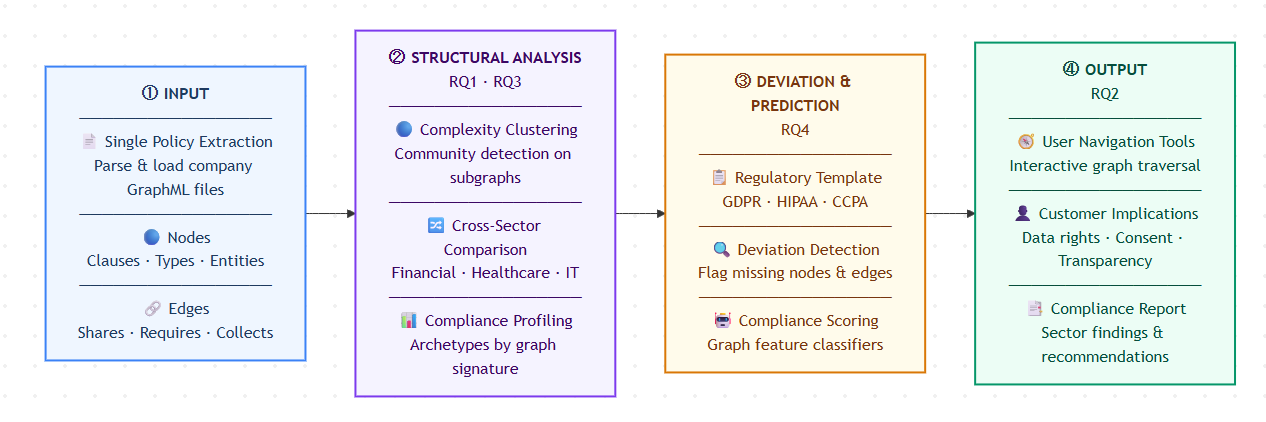
\includegraphics[width=\textwidth]{Framework.png}
    \caption{Proposed four-stage knowledge graph framework for privacy policy compliance analysis.}
    \label{fig:framework}
\end{figure*}


In the second stage, graph-theoretic methods are applied to perform structural analysis, encompassing complexity clustering through community detection algorithms, cross-sector schema comparison to surface divergence in policy architecture, and compliance profiling to classify organizations into archetypes based on their graph signatures, collectively addressing RQ1 and RQ3. 

The third stage introduces a deviation and prediction layer, in which regulatory reference graphs derived from established frameworks such as the General Data Protection Regulation (GDPR), the Health Insurance Portability and Accountability Act (HIPAA), and the California Consumer Privacy Act (CCPA) serve as compliance benchmarks; graph feature classifiers are then trained to detect structural deviations and generate compliance scores per-company, addressing RQ4. 

Finally, the fourth stage translates graph-level findings into interpretable outputs, including user navigation tools designed to enable non-technical stakeholders to traverse policy graphs, and actionable insights surfacing gaps in data rights, consent transparency, and user protections, thereby addressing RQ2. Collectively, this framework leverages the relational expressiveness of knowledge graphs to move beyond flat-text policy analysis, enabling structured, comparative, and predictive reasoning over privacy policy language at scale.

\section{Literature Review}

POLIGRAPH \cite{cui2023} is a knowledge graph architecture developed by Cui et al. (2023) to address the shortcomings of sentence-level privacy policy (PP) analyzers, which lack the ability to capture global structural relationships and cross-sentence dependencies. The authors built POLIGRAPH-ER, an NLP pipeline that uses dependency parsing, named entity recognition (NER), and ontology-based reasoning to extract relational information from policy documents as a whole. Their knowledge graph model represents data types, entities, purposes, and their relationships through subsumption and collection relationships. POLIGRAPH demonstrates 97\% precision and identifies 40\% more statements of data collection than existing systems, as claimed in their evaluation. This makes it possible to check whether actual data practices follow the privacy policy and to identify statements in the policy that contradict each other. The primary limitations are that the system only analyzes data collection (not sharing or storage) and performs poorly on tables, ambiguous language, and rare sentence patterns.

The paper by Yerby et al. \cite{yerby2022} examines how corporations intentionally craft confusing Terms of Service (TOS) and Privacy Policies (PP) to obscure data‑handling practices. Through legal analysis and real‑world examples, the authors highlight the lack of regulatory standards governing readability and transparency. They argue for federal reforms modeled after successful consumer‑protection legislation, such as the Fair Credit and Charge Card Disclosure Act. While the paper provides strong conceptual grounding, it lacks computational methods and empirical evaluation, making it complementary but methodologically distinct from the other studies.

Ramasamy et al. \cite{ramasamy2025} focuses on using clustering-based structural analysis and interactive graph visualizations to improve the interpretability of PP. To create node embeddings, the authors use dimensionality-reduction techniques (t-SNE, UMAP, and PCA) and build KGs for 55 Android e-commerce apps using PoliGraph-ER. Multiple clustering techniques, such as Mini-Batch K-Means, Agglomerative Clustering, HDBSCAN, Spectral Clustering, and LDA, are then evaluated. According to the results, the best separation is obtained when t-SNE and spectral clustering are combined. This reveals important communities including Media & Location, Device Information, and User Activity. Assessments of regulatory compliance and forensic investigations are supported by these findings. Two of the dataset's limitations include its modest size and the lack of semantic extraction beyond structural grouping.

Barrett et al \cite{barrett2025} explores how NLP and knowledge graph techniques can simplify PPs and flag potential privacy risks. The authors scrape PP URLs from top Android e‑commerce apps and process them through two KG pipelines: a baseline n‑gram–based PoliGraph‑ER and a modified skip‑gram–based version. The skip‑gram model captures broader contextual relationships, improving semantic linkage between PP terms. The framework supports automated summarization, risk identification, and user‑centric transparency. Despite its contributions, the study lacks quantitative evaluation of skip‑gram improvements and relies on a relatively small dataset of 100 e-commerce shopping apps.


Joshi et al. \cite{joshi2020} addresses the problem that corporations face with the varied and complex privacy and data protection rules relating to cloud data storage and computing. They seek to support businesses in automating data compliance and developing a real time violation detection Knowledge Graph that can ingest data compliance regulations and identify threats and security controls. The team methods include data identification of privacy laws and regulations. They leverage Knowledge Graph with OWL (Web Ontology Language) and RDF (Resource Description Framework) to represent the data. Their data extraction focuses on GDPR Knowledge Graph, PCI DSS, and Cloud Security which includes chapter extraction and key term and class identification. They validate on company websites including Amazon, Google, IBM and Rackspace against real world privacy policies like NIST SP 800-53, plus compliance models for cloud computing. A key finding and contribution is that privacy policy data scraped from the web can be converted to a machine processable format via a RDF graph. Other contributions are the real-time identification and mapping from threat to control for potential real-time mitigation. Finally, language context is known due to semantic reasoning, so that a duplicated regulation in two different policies can be identified as the same. A limitation or gap is that not all privacy and data protection policies are included. 

Belcheva et al. \cite{belcheva2023} addresses a key limitation in prior privacy policy research, which often examines policies at a single point in time or within a narrow domain such as healthcare. This study expands the scope by analyzing data privacy and protection policies from 2000 to 2019, across a broad range of organizations. The authors find that privacy policies have become increasingly difficult to read and more vague over time. They also identify a growing trend of reassuring or pacifying language while overall readability declines. This may signal attempts to create a false sense of security despite reduced clarity. The authors extract data and clean sentences; they categorize websites, identify GDPR-related policies, and compute readability metrics, assess vagueness, and train a BERT classifier to label sentences. They also detect reassuring or positive phrases and analyze trends over time, across domains, and in relation to GDPR content, supplemented by outlier analysis and manual review. The findings from this analysis challenge corporations to provide more transparent, less vague, and more concise and readable privacy policies. 
Limitations or gaps are that the dataset does not extend past 2019. Also, the size of the dataset could be a challenge for processing time. 

In "PrivComp-KG: Leveraging KG and LLM for Compliance Verification," Garza et al. \cite{garza2024} observe that privacy and data protection regulations are complex and long, making it difficult for organizations to remain in compliance. This is further complicated because vendors who help manage privacy policy documentation and updates sometimes provide insufficient detail. To address this problem, Garza et al.\cite{garza2024} developed a Privacy Compliance Verification Knowledge Graph tool (PrivComp-KG) to store and retrieve privacy policy data with LLM and Retrieval Augmented Generation (RAG). This tool then maps privacy policies relevant to the sector or situation and maps to the relevant regulation. 
The accuracy levels are high, outperforming other models, with a correctness score of 0.9. The domain and regulation knowledge can then be queried to assess compliance and identify and address gaps in privacy policies. This study is limited to specific GDPR sections and may not include modern updates. Further, there is no process for real-time updates for changing laws. 

Chowdhury et al.\cite{Chowdhury2026} in GraphDPR proposes a framework to analyze e-commerce privacy policies by converting unstructured privacy policy text into structured knowledge graphs to improve interpretability. The methodology combines transformer-based natural language processing with Neo4j Knowledge Graph construction, Sentence-BERT embeddings for semantic normalization, and Latent Dirichlet Allocation to identify thematic patterns. The evaluation focuses on metrics such as regulatory coverage, semantic interpretability, and topic clarity when compared with prior systems. A key strength of the approach is its visualization of relationships among entities, data types, and policy actions. GraphDPR extends POLIGRAPH and highlights company specific behaviours (like financial disclosures) and shared norms (such as contact and tracking data). Limitations and future work includes embedding privacy policy clauses for rule-based auditing. 



\section{Conclusion}

The reviewed literature reveals three major trends in privacy policy analysis. First, there is a clear shift from sentence-level analysis to document-level structural understanding, exemplified by POLIGRAPH's knowledge graph approach and GraphDPR \cite{cui2023} \cite{joshi2020} \cite{Chowdhury2026}. Second, researchers increasingly recognize that privacy policy complexity is not merely a technical challenge but often a deliberate obfuscation strategy \cite{yerby2022}\cite{belcheva2023}. Third, there is growing emphasis on visualization and clustering techniques to make complex policy structures interpretable \cite{ramasamy2025, barrett2025}.  

Joshi et al. \cite{joshi2020} A key finding and contribution is that privacy policy data scraped from the web can be converted to a machine processable format. This issue must be addressed for our study.  Other contributions are the real-time identification and mapping from threat to control for potential real-time mitigation. 

Current research leaves critical questions unanswered. Existing tools are able to assess individual privacy policies \cite{cui2023, ramasamy2025, barrett2025}, but they are unable to compare the differences in compliance between the IT, healthcare, and financial sectors or identify patterns peculiar to them (RQ1). However, PrivComp-KG and GraphDPR does show promise in this area with its sector mapping \cite{garza2024} \cite{Chowdhury2026}. Moreover, no study looks at how these compliance discrepancies actually effect customers in real-world situations, particularly how policy variances impact transparency, user rights accessibility, and data protection capability (RQ2).
While Ramasamy et al. \cite{ramasamy2025} applied clustering to individual apps, no work investigates whether structural analysis can reveal meaningful compliance patterns across entire industries, such as identifying "privacy-protective" versus "minimally compliant" industry groups (RQ3). Additionally, no framework currently employs predictive models to automatically identify policies that deviate from regulatory expectations or industry norms, limiting regulatory oversight capabilities (RQ4). These gaps are compounded by small dataset limitations, with studies using only 55-100 policies from single domains \cite{ramasamy2025, barrett2025}, insufficient for meaningful cross-industry pattern analysis. A large dataset was used in Joshi et al,, but it is based on actual policies, not regulations, and is not a modern dataset (post 2019). \cite{joshi2020} 

To address RQ1, we plan to build knowledge graphs from policies across financial, healthcare, and IT sectors and compare their data handling practices to reveal sector-specific patterns. For RQ2, we will translate these technical differences into practical customer impacts regarding data protection, user rights, and transparency. For RQ3, we plan to apply clustering techniques \cite{ramasamy2025} to identify compliance patterns across industries. For RQ4, we will train predictive models on regulatory frameworks (GDPR, HIPAA, CCPA) to automatically flag policy deviations and potential violations \cite{yerby2022}. Our framework will combine knowledge graph construction \cite{cui2023, barrett2025}, structural clustering \cite{ramasamy2025}, and obfuscation detection \cite{yerby2022} to enable cross-industry comparative analysis, helping users identify privacy-protective companies and supporting regulatory oversight.



\bibliographystyle{ieeetr}
\bibliography{references}


\end{document}
